\chapter{Analysis}
% Lav analyse af hvad der er nu ( data) og hvad kan jeg bruge det til
% Hvad KAN jeg bruge det til og hvad vil jeg bruge det til

% Diskuter problematikken om at man gerne vil lave tekniske ting, der skal bruges af ikke-tekniske mennesker

In this chapter, I will present and analyze the data made available by the MCP in the three documents \ttt{E2 - NW-NM DMA Service Instance}, \ttt{E2 - NW-NM REST Service Technical Design}, and \ttt{E2 - NW-NM Service Specification}, which represent all data, made available to me. Furthermore, I will explain the necessity of testing the MCP, as well as present a description of a favorable model structure. 

\section{Data} % hvad er tilgængeligt nu?

To provide a holistic description of a service instance, three documents are necessarily provided. Below are the descriptions of the documents with the service instance \ttt{E2 - NW-NM DMA} as an example.
\begin{itemize}
	\item \ttt{E2 - NW-NM DMA Service Instance} \\
	The purpose of this service instance document and its xml-defined counterpart is to describe a DMA instance of the REST-based technical design of the MW- NM service specification, according to the guidelines given in the Service Description Guidelines.
	\item \ttt{E2 - NW-NM REST Service Technical Design} \\
	The purpose of this service technical design document and its xml-defined counterpart is to describe a REST-based technical design of the MW-NM service specification, according to the guidelines given in the Service Description Guidelines.
	\item \ttt{E2 - NW-NM Service Specification} \\
	The purpose of this service specification document and its xml-defined counterpart is to provide a holistic overview of the MW-NM service and its building blocks in a technology-independent way, according to the guidelines given in the Service Description Guidelines.
\end{itemize}

Of the three documents, only the last, \ttt{Service Specification} is to be used to describe specifications of the service, and as such only this will be studied closer.
\section{Service Specification grammar}
The service specification document is constructed using a general xml-format. The grammar of the document can be seen in Listing \ref{lst:sSpecFull} as well as in Listing \ref{lst:sSpecReduced}, while the latter is in a severely reduced and generalized form.
\begin{lstlisting}[mathescape=true, keywordstyle={},label={lst:sSpecFull},caption={Full parser grammar of Service Specification Schema},captionpos={below}]
ServiceSpecificationSchema ::= specifications

specifications ::= spec specifications
     | $\epsilon$
     
spec ::= name
     | status
     | id
     | version
     | description
     | keywords
     | isSpatialExclusive
     | authorInfos
     | requirements
     | serviceDataModel
     | serviceInterfaces
     
authorInfos ::= authorInfo authorInfos
     | $\epsilon$

authorInfo ::= aSpec authorInfo
     | $\epsilon$

aSpec ::= id
     | name
     | description
     | contactInfo

requirements ::= requirement requirements
     | $\epsilon$

requirement ::= rSpec requirement
     | $\epsilon$

rSpec ::= id
     | name
     | text

serviceDataModel ::= definitionAsXSD

definitionAsXSD ::= $\epsilon$

serviceInterfaces ::= serviceInterface serviceInterfaces
     | $\epsilon$

serviceInterface ::= siSpec serviceInterface
     | $\epsilon$

siSpec ::= name
     | description
     | dataExchangePattern
     | operations

operations ::= operation operations
     | $\epsilon$

operation ::= oSpec operation
     | $\epsilon$

oSpec ::= name
     | description
     | returnValueType
     | parameterTypes

returnValueType ::= typeReference


parameterTypes ::= parameterType parameterTypes
     | $\epsilon$

parameterType ::= ptSpec parameterType
     | $\epsilon$

ptSpec ::= typeReference
\end{lstlisting}

\begin{lstlisting}[mathescape=true, keywordstyle={}, label={lst:sSpecReduced}, caption={Reduced parser grammar of Service Specification Schema},captionpos={below}]
ServiceSpecificationSchema ::= specifications

specifications ::= spec specifications
     | $\epsilon$
     
spec ::= specifications
     | spec
     | $\epsilon$
\end{lstlisting}

As mentioned above, the service specification is to be used to verify the behavior of the maritime service from a technical stand point. At the moment, the xml-document provides a technical description of its corresponding maritime service, but the most commonly used expression method is free text. As this is a very non-technical design choice, a large portion of the obvious technical advantages, provided by the xml-format are lost. 

% Skal jeg have mere ind her? om hvordan det kan ændres til noget smartere, eller skal jeg gemme det til 'work'

The xml-version of the service specification can be found in appendix \ref{sec:E2 - NW-NM Service Specification}.

\section{Testing the MCP} % Why do we want to test/validate

The core principle in the MCP is to restructure and streamlining maritime software sharing in a manner that can be done the world over, and the very nature of this statement dictates that the platform must be highly scalable. This adds the necessity of running quality-checks on all of the maritime services that are uploaded to the platform. To accommodate this issue, model-based testing immediately seems like the obvious solution, as this technique covers most of the required desired functionality. If implemented satisfyingly, a model-based testing suite for the MCP would be able to
\begin{enumerate}
	\item Present or verify behavior of maritime services.\\
	There are many obvious common behavioral traits of maritime services, such as adding ships and maritime stakeholders, as well as removing them, however other behavioral patterns will often vary to the point of lowered manageability. A model, describing the maritime service in question will provide a clear and undeniable description of the service's behavior.
	\item Visualize functionality of maritime services.\\
	Just as well as behavioral traits, functionality will differ greatly from one maritime service to another, and therefore it is very useful for a model to visualize said functionality, as well as verifying that it works as intended.
	\item Present the structures of maritime services.\\
	This trait will be used to visualize the structural components of maritime services. Just as point 1 and two, this functionality will be useful for creating a quick and clear projection of how the maritime service behaves.
	\item Increase reliability and efficiency of maritime services.\\
	Through correct implementation of points 1-3 it is possible to elevate the reliability and efficiency of the maritime services found on the MCP. This is due to the same reasoning that all testing is conducted on the basis of: the need for safe, consistent, and correct code.
\end{enumerate}

As stated in Section \ref{sec:Model-Based Testing} there are two main types of model-based testing techniques: serial and sequential model building-and testing. 

% Hvordan kan man teste dette?

\section{Model Structure} % Hvordan ville en model ideelt se ud?

\begin{figure}[H]
	\centering
	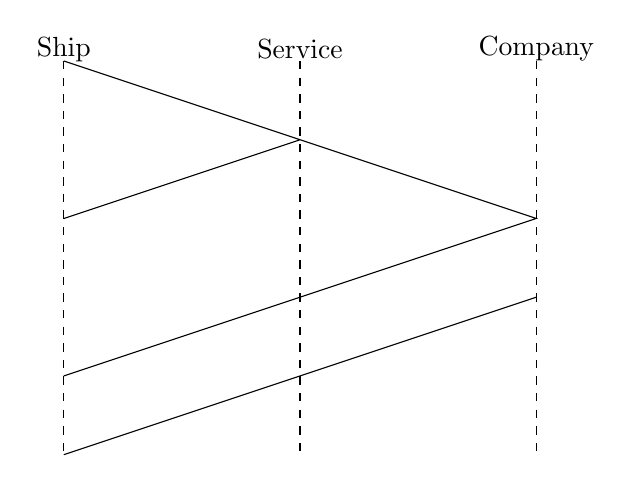
\begin{tikzpicture}
		
		% timelines
		\draw	[dashed] (0,5) -- (0,0)
				[dashed] (3,5) -- (3,0)
				[dashed] (6,5) -- (6,0);

		% labels
		\draw	(0,5.15)	node	{Ship}
				(3,5.15)	node	{Service}
				(6,5.15)	node	{Company};

		% interaction lines
		\draw	(0,5) -- (3,4) -- (0,3)			% API call (request/response)
				(3,4) -- (6,3) -- (3,2) -- (0,1)% Service requests/recieves data from company/data center
				(6,2) -- (3,1) -- (0,0);		% Additional line
	\end{tikzpicture}
	\caption{Rough draft of a model example, where a ship requests something from a service (could be a weather update)}
	\label{fig:modelEx}
\end{figure}

% i XML'en:
%	lav et felt, der hedder entitet
%		definer relation, rolle, etc
%	definer videre på roller, hvad vil de have fra hinanden?
%	


% definér en protokol
% byg på eksisterende entiteter
% 
% vejrudsigt-service
% fra vejrservicens perspektiv:
% et skib anmoder om oplysninger, hvilken informationer skal skibet videregive for at blive tildelt oplysninger
% 
% meget lavpraktisk model:
% tre foruddefinerede modeller, der snakker med hinanden. Simulér en interaktion mellem dem - hvordan skifter de forskellige tilstand når de interagerer?
% hvilke reaktioner kommer der på aktioner?
% opfører en entitet sig rigtigt i forhold til en anden entitet når de interagerer på en bestemt måde?
% 
% kan GODT lave drop down menuer i nye xml-filer

\section{Model-Based testing of MCP} % Hvad kan man teste med dette?

\section{Issues} %Problematikker: F.eks at folk, der lægger software op ikke nødvendigvis selv kan lave modellerne/forstå at give argumenterne, der skal bruges til at generere modeller automatisk